% chap2.tex (Definitions)

\chapter{Background and Related Work}\label{background}

This section outlines some of the state of the art in the area of data provenance for file systems, data compression techniques for data provenance, and intrusion detection using data provenance.

\section{Overview of Provenance Aware systems}

There has been a considerable amount of work done on collecting provenance data. Some of which has been focused on databases, sensor networks and system level provenance but so far little attention has been given to provenance in IoT devices. Some the previous work done on data provenance collection are outlined below:

\subsection{Provenance Aware Storage System(PASS)}
MuniswamyReddy
et al developed a proveenance aware system that tracks provenance of the linux file system. There are two versions PASS v1 and PASS v2. v1 allows... while version 2...Provenance information
is stored in the same location as the file system for easy accessibility, backup,
restoration, and data management. Provenance information is collected and stored in
the kernel space. The system also provides provenance query capabilities and cycle
detection. PASS systems recognizes data pruning for efficient storage, which is in line
with our research goal but data pruning was not fully explored in PASS.

The collector keeps track of system level provenance. It intercepts system calls which are translated into provenance data and is stored in an in kernel database. This database maps key value pairs for provenance data for fast index look up. It also provides functionalities for querying provenance data in the database. PASS detects and eliminates cycles that might occur in provenance dependencies as a result of version avoidance.cycles violates the dependency relationships between entities. For example, a child node could depend on a parent node and also be an ancestor of a parent node. It achieves this by merging processes that might have led to the cycles.

\subsection{HiFi}
Bates et al. [2] developed system level provenance information for the Linux kernel using a Linux Provenance Modules, which tracks whole system provenance including interprocess communication, networking, and kernel activities. This is achieved by mediating access to kernel objects. Linuex Security Model is a framework that was designed for providing custom access control into the Linux kernel.It consists of a set of hooks which is executed before access decision is made.

HiFi contains three components, provenance collector, provenance log and provenance handler. collector and log are in the kernel space while the handler is in the user space.The log is a storage medium which transmits the provenance data to the user space.The collector contains the LSM which resides the kernel space. The collector records provenance data and writes it to the provenance log.The handler intercepts the provenance record fromt he log processes the data and stores it to the provenance record. LSM was designed to avoid problem created by direct system call interception. The provenance information from the kernel space is securely transmitted to the provenance recorder in the user space. This approach to collecting provenance data differs from our work since we focus on embedded systems and are concerned with input and output (I/O) data, which primarily involve sensor and actuator readings.

\subsection{RecProv}

creates a provenance system which records user level provenance thereby avoiding the overhead incurred by kernel level provenance recording.It uses mozilla rr to perform deterministic record and replay by capturing system calls  and non deterministic input. It also ensure the integrity of provenance data up till the point that the host is compromised by trace isolation. Mozilla rr relies on ptrace which intercepts system call during context switch.Mozilla rr is a debugging tool for linux browser. It is developed for the deterministic recording and replaying of firefox browser in linux. System calls such as execve, clone, fork, open, read, write, clode, dup, mmap, socket, connect, accept are recorded. the provenance information generated in converted into PROV-JSON a W3C standard for relaying provenacne information and also stores provenance data in Neo4j a graph database for visualization of provenance graphs. It does not require changes to the kernel like most provenance monitoring systems (include citations of other provenance monitoring systems that require kernel modification). it generates 20 percent overhead which is acceptable according to the authors.

Recprov uses PTRACE\_PEEKDATA from PTRACE to access the derefrenced address of the traced process from the registers.

\subsection{StoryBook}
Spillance et al developed a user space provenance collection system, Storybook \cite{Rabinovich1995}  that allows the collection of provenance data from the user space thereby reducing performance oververhead from kernel space provenance collection. This system is modular.It allows the use of application specific extensions allowing additions such as database provenance, system provenance, and web and email servers. It achieves provenance capture by using FUSE for system level provenance and MYSQL for database level provenance capture. Story Book allows developers to implememtn provenance inspectors. these are custom provenance models which captures the provenance of applications which are often modified by different application(e.g web servers, databases). When an operation is performed on a data object, the appropriate provenance model is triggered and provenance data for that data object is captured. Sotrybook stores provenance information such as open, close, read or write, application specific provenance, causality relationship between entities contained in the provenance system(?). Provrenance is stored in key value pairs and It uses Fable as the storage backend. Storybook allows for provenance query.It achieves this by looking up inode in the file, ino hashtable.

\subsection{Trustworthy whole system provenance for Linux kernel}

\subsection{Towards Automated Collection of Application-Level Data Provenance}

\subsection{user space provenance with Sandboxing}
\

\subsection{Provenance for Sensors}
Lim et al. [3] developed a
model for calculating the trust of nodes contained in a sensor network by using data
provenance and data similarity as deciding factors to calculate trust. The value of
provenance signifies that the more similar a data value is, the higher the trust score.
Also, the more the provenance of similar values differ, the higher their trust score.
This work differs from our approach since the authors focus on creating a trust score
of nodes connected in a sensor network using data provenance and do not emphasize
how the provenance data is collected. We are focused on creating a secure
provenance aware system for I/O operations which is used to ensure trust of
connected devices.




\section{Model for representing provenance for IoT}

In order to generate provenance, we have to satisfy the who, where, how, and what of data transformations.provenance data is represented using a provenance model which is serialized as JSON output. This model contains information such as sensor readings, device name,, device information, provenance information. This information will be converted into provenance data model and in order to allow for interoperability and visualization.

\subsection{Open Provenance Model(OPM)}

Open provenance model was a specification derived as a result of a meeting at the International Provenance and Annotation Workshop (IPAW) workshop in may 2006. OPM was created to address the need of allowing a unified way of representing provenance data among various applications. It allows for interchangeability between various provenance models that might exist. The goal of OPM is to develop a digital representation of provenance for entities regardless of whether it is produced by a computer system. An example of such is depicted in Figure 7. This OPM graphs represents a process of driving a car. It is represented as a directed acyclic graph which denotes causal dependencies between entities. The edges in the graph denotes dependencies with its source denoting effect and its destination denoting cause.The edges and their relationships are denoted below: 

When muliple process has been used by an artifact, roles(denopted by R) should be defined.

\begin{itemize}
\item wasGeneratedBy: Shows relationship in which an entity(e,g artifact) is utilized by one or  more entities(e.g process). An entity can use multiple enities so it is important to define the role of the  
\item wasControlledBy: This showsa the relationship in which an entity caused the creation of another entity.
\item used(Role): denotes an enity requires the services of another enity in order to execute.
\item wasTriggeredBy: 
\item wasDerrivedFrom:
\end{itemize}

 There are three entities contained in the OPM model: artifact, process, agent. 

\begin{itemize}
\item
artifact: This represents the state of an entity.An artifact is graphically represented by a circle.

\item
Process: This denotes an event which is taking place.A process is represented by a square object.

\item 
Agent: These are actors that facilitate the execution of a process.An agent is represented by a hexagon.
\end{itemize}

OPM denotes all previous and current actions that have been performed on an entity and  the relationship between each entities contained in the graph. Figure 2 represents an example of an OPM acyclic graph with all of its causal dependencies. The goal of OPM is to be able to model the state of how things both digital or physical are at a given state.   

\begin{figure}[h!]
\begin{center}

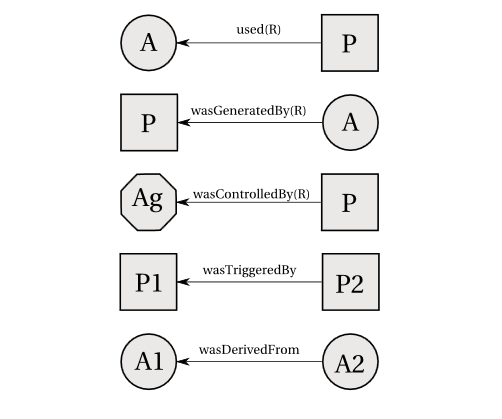
\includegraphics{opm_convention.PNG}
\end{center}
\caption{Edges and entities in OPM}
\label{autom}
\end{figure}

%\begin {center}
%\begin {tikzpicture}[-latex ,auto ,node distance =4 cm and 5cm ,on grid ,
%semithick ,
%state/.style ={ circle ,top color =white , bottom color = processblue!20 ,
%draw,processblue , text=blue , minimum width =1 cm}]
%\node[state] (C)
%{$1$};
%\node[state] (A) [above left=of C] {$0$};
%\node[state] (B) [above right =of C] {$2$};
%\path (A) edge [loop left] node[left] {$1/4$} (A);
%\path (C) edge [bend left =25] node[below =0.15 cm] {$1/2$} (A);
%\path (A) edge [bend right = -15] node[below =0.15 cm] {$1/2$} (C);
%\path (A) edge [bend left =25] node[above] {$1/4$} (B);
%\path (B) edge [bend left =15] node[below =0.15 cm] {$1/2$} (A);
%\path (C) edge [bend left =15] node[below =0.15 cm] {$1/2$} (B);
%\path (B) edge [bend right = -25] node[below =0.15 cm] {$1/2$} (C);
%\end{tikzpicture}
%\end{center}

\subsection{Provenance Data Model(ProvDM)}

PROV-DM is a W3C standardized extension of OPM. Prov-DM is a model that is used for depict causal relationship between entities, activities and , and agents(digital or physical).  It creates a common model that allows for interchange of provenance information between heterogeneous devices. It contains two major components: types and relations. Figure below shows an example of a causal relationship between an entity, agent, and activity in a PROV-DM

\begin{itemize}

\item entity: An entity is a physical or digital object. An example of an entity is a file system, a process, or an motor vehicle.

\item Activity: An activity represents some form of action that occurs over a time frame.Actions are acted upon by an entity. an example of an activity is a process opening a file directory, Accessing a remote server.

\item Agent: An agent is a thing that takes ownership of an entity, or performs an activity. An example of an agent is a person, a software product, a process.
\end{itemize}

PROV-DM relations represents causal dependencies which denotes relationship between the core types(entity, activity, agent).The names of relations make use of past tense to denote past occurrence of provenance information. provenance does not keep track/estimate of future events. PROV relations are outlined below:


\begin{itemize}
\item wasGeneratedBy: This relation signifies the creation of an entity by an activity. 

\item used: This relation denotes that the functionalities of an entity has been adopted by an activity.

\item wasInformedBy: This relation denotes an causality that follows the exchange of two activities.

\item wasDerievedFrom This relation represents a copy of information from an entity. 

\item wasAttributedTo: This denotes relational dependency to an agent. It is used to denote relationship between entity and agent when the activity that created the agent is unknown.

\item wasAssociatedWith:This relation denotes a direct association to an agent for an activity that occurs.This indicates that an agent plays a role in the creation or modification of the activity.

\item ActedOnBehalfOf: This denotes assigning authority to perform a particular responsibility to an agent. This could be by itself or to another agent.



\end{itemize}

Prov-DM contains similar yet subtle differences between OPM.Some of the difference between OPM and PROV-DM are outlined below:

\begin{itemize}

\item the main components Artifact, process and agent in the OPM model are changed to Entity, Action, and agent. 

\item additional causal dependencies such as wasAttributedTo and actedOnBelafOf are included to represent direct and indirect causal dependencies respectively between agents and entity.

\end{itemize}


Entities, activities and agent are represented by oval, rectangle and hexagonal shape respectively.
Since PROV-DM is built on OPM and contains easy to understand constructs of enities, we choose to use this instead of OPM. 


\section{Overview of Data pruning techniques}

\subsection{Graph Compression}

\subsection{Dictionary Encoding}

\subsection{Arithmetic Encoding}


\section{Intrusion Detection for IoT}



%%% Local Variables: 
%%% mode: latex
%%% TeX-master: "thesis"
%%% End: 
